\documentclass{article}
\usepackage{tikz}
\usetikzlibrary{shapes, shapes.multipart, shapes.symbols, shapes.geometric, shapes.misc, positioning, fit, backgrounds, arrows.meta, calc}
\usepackage[margin=0.8in]{geometry}
\usepackage{titlesec}
\usepackage{fancyhdr}

% Professional Formatting
\titleformat{\section}{\large\bfseries}{\thesection}{1em}{}
\pagestyle{fancy}
\fancyhf{}
\rhead{Social Help and Donation System}
\lhead{Technical Documentation}
\cfoot{\thepage}

\begin{document}

\begin{titlepage}
    \centering
    \vspace*{2cm}
    {\Huge\bfseries Social Help and Donation Management System\par}
    \vspace{1cm}
    {\Large\bfseries Technical Documentation Suite\par}
    \vspace{2cm}
    {\large Prepared for Project Review\par}
    \vfill
    {\large \today \par}
\end{titlepage}

\tableofcontents
\newpage

% ---------------------------------------------------------
\section{Use Case Diagram}
% -------------------------
\begin{figure}[htbp]
\centering
\resizebox{0.9\textwidth}{!}{
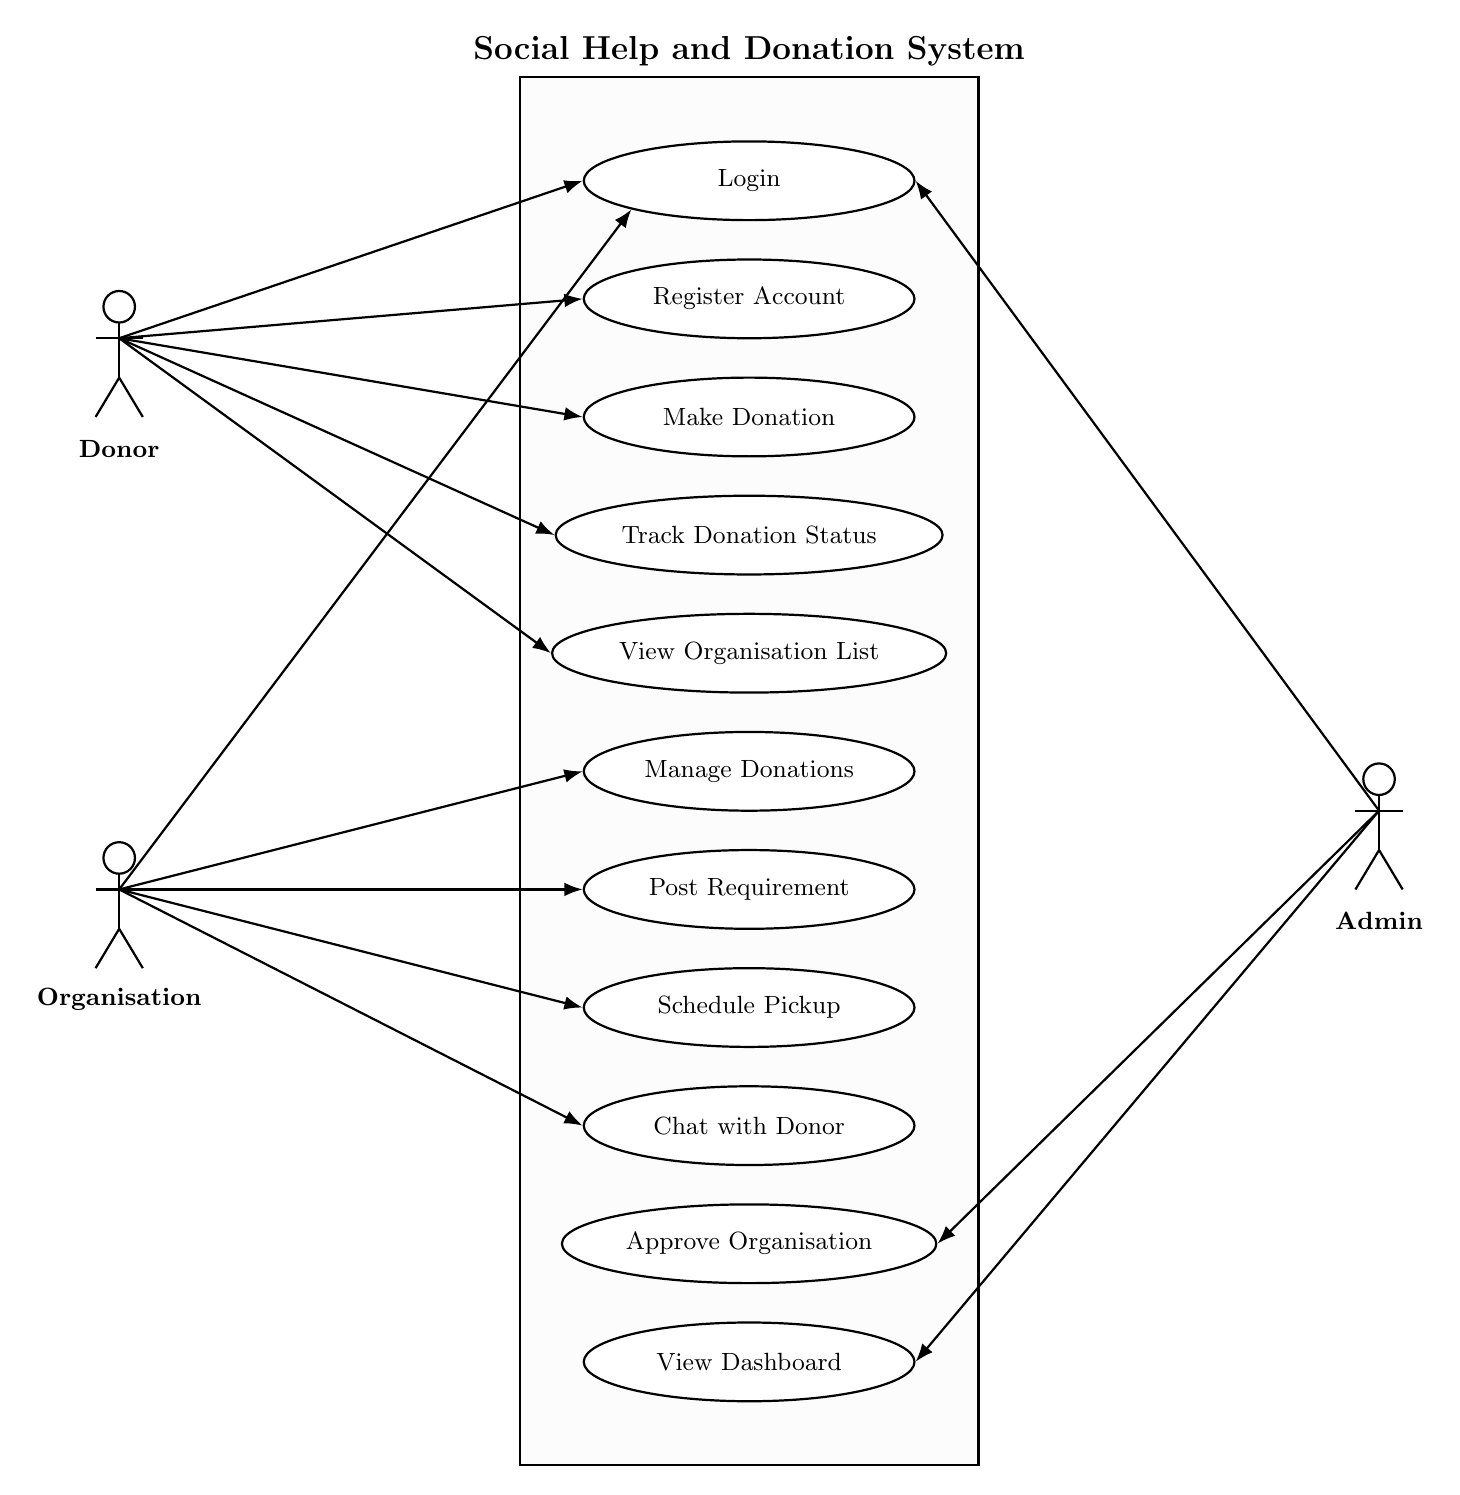
\begin{tikzpicture}[
    >=Latex, thick,
    actor/.style={align=center, font=\small\bfseries},
    usecase/.style={draw, ellipse, minimum width=4.2cm, minimum height=1cm, align=center, fill=white, font=\small}
]
\tikzset{
    stickman/.pic={
        \coordinate (-chest) at (0, 0);
        \draw[thick] (0, 0.4) circle (0.2);
        \draw[thick] (0, 0.2) -- (0, -0.5);
        \draw[thick] (-0.3, 0) -- (0.3, 0);
        \draw[thick] (0, -0.5) -- (-0.3, -1);
        \draw[thick] (0, -0.5) -- (0.3, -1);
    }
}
\node[usecase] (UC1)  at (0,  7.5) {Login};
\node[usecase] (UC2)  at (0,  6.0) {Register Account};
\node[usecase] (UC3)  at (0,  4.5) {Make Donation};
\node[usecase] (UC4)  at (0,  3.0) {Track Donation Status};
\node[usecase] (UC5)  at (0,  1.5) {View Organisation List};
\node[usecase] (UC6)  at (0,  0.0) {Manage Donations};
\node[usecase] (UC7)  at (0, -1.5) {Post Requirement};
\node[usecase] (UC8)  at (0, -3.0) {Schedule Pickup};
\node[usecase] (UC9)  at (0, -4.5) {Chat with Donor};
\node[usecase] (UC10) at (0, -6.0) {Approve Organisation};
\node[usecase] (UC11) at (0, -7.5) {View Dashboard};
\begin{scope}[on background layer]
    \node[draw, rectangle, thick, fill=gray!2, inner sep=0.8cm, fit=(UC1)(UC11)] (System) {};
    \node[anchor=south, font=\large\bfseries] at (System.north) {Social Help and Donation System};
\end{scope}
\pic (DonorPic) at (-8,  5.5) {stickman}; \node[actor] at (-8, 4.1) {Donor};
\pic (OrgPic) at (-8, -1.5) {stickman}; \node[actor] at (-8, -2.9) {Organisation};
\pic (AdminPic) at (8, -0.5) {stickman}; \node[actor] at (8, -1.9) {Admin};
\draw[->] (DonorPic-chest) -- (UC1.west);
\draw[->] (DonorPic-chest) -- (UC2.west);
\draw[->] (DonorPic-chest) -- (UC3.west);
\draw[->] (DonorPic-chest) -- (UC4.west);
\draw[->] (DonorPic-chest) -- (UC5.west);
\draw[->] (OrgPic-chest) -- (UC1.south west);
\draw[->] (OrgPic-chest) -- (UC6.west);
\draw[->] (OrgPic-chest) -- (UC7.west);
\draw[->] (OrgPic-chest) -- (UC8.west);
\draw[->] (OrgPic-chest) -- (UC9.west);
\draw[->] (AdminPic-chest) -- (UC1.east);
\draw[->] (AdminPic-chest) -- (UC10.east);
\draw[->] (AdminPic-chest) -- (UC11.east);
\end{tikzpicture}
}
\end{figure}

\newpage
% ---------------------------------------------------------
\section{UML Class Diagram}
% -------------------------
\begin{figure}[htbp]
\centering
\resizebox{0.95\textwidth}{!}{
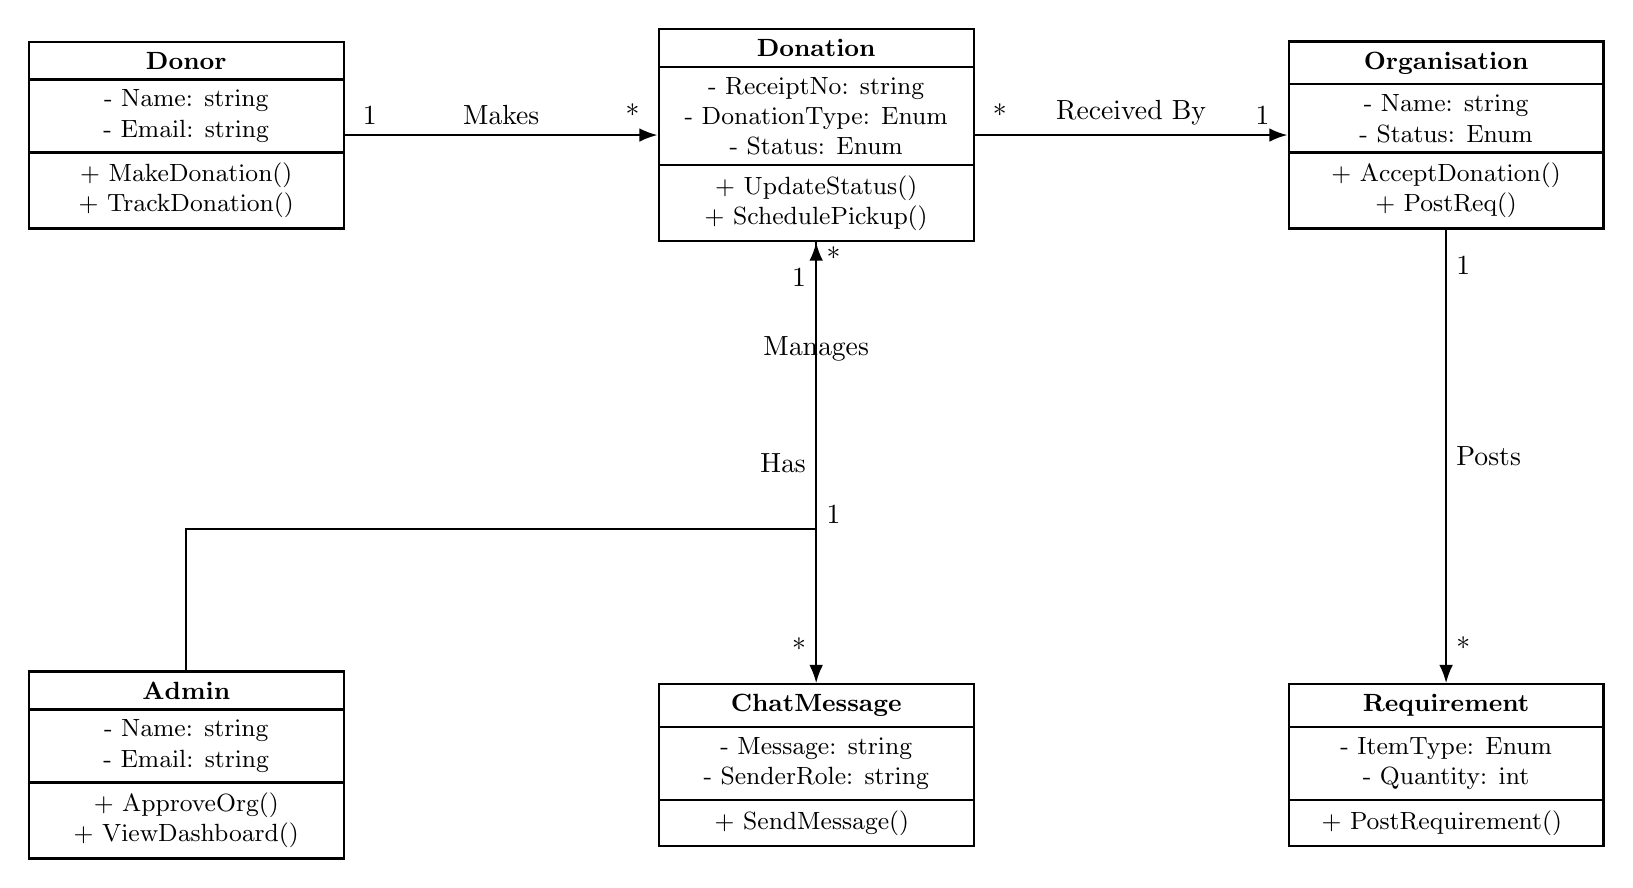
\begin{tikzpicture}[
    >=Latex,
    class/.style={draw, rectangle split, rectangle split parts=3, minimum width=4cm, align=center, fill=white, thick, font=\small}
]
\node[class] (Donation) at (0, -1) { \textbf{Donation} \nodepart{second} - ReceiptNo: string \\ - DonationType: Enum \\ - Status: Enum \nodepart{third} + UpdateStatus() \\ + SchedulePickup() };
\node[class] (Donor) at (-8, -1) { \textbf{Donor} \nodepart{second} - Name: string \\ - Email: string \nodepart{third} + MakeDonation() \\ + TrackDonation() };
\node[class] (Organisation) at (8, -1) { \textbf{Organisation} \nodepart{second} - Name: string \\ - Status: Enum \nodepart{third} + AcceptDonation() \\ + PostReq() };
\node[class] (Admin) at (-8, -9) { \textbf{Admin} \nodepart{second} - Name: string \\ - Email: string \nodepart{third} + ApproveOrg() \\ + ViewDashboard() };
\node[class] (ChatMessage) at (0, -9) { \textbf{ChatMessage} \nodepart{second} - Message: string \\ - SenderRole: string \nodepart{third} + SendMessage() };
\node[class] (Requirement) at (8, -9) { \textbf{Requirement} \nodepart{second} - ItemType: Enum \\ - Quantity: int \nodepart{third} + PostRequirement() };

\draw[->, thick] (Admin.north) -- (-8, -6) -- (0, -6) -- (Donation.south) node[pos=0.05, right] {1} node[pos=0.55, above] {Manages} node[pos=0.95, right] {*};
\draw[->, thick] (Donor.east) -- (Donation.west) node[pos=0.08, above] {1} node[midway, above] {Makes} node[pos=0.92, above] {*};
\draw[->, thick] (Donation.east) -- (Organisation.west) node[pos=0.08, above] {*} node[midway, above] {Received By} node[pos=0.92, above] {1};
\draw[->, thick] (Donation.south) -- (ChatMessage.north) node[pos=0.08, left] {1} node[midway, left] {Has} node[pos=0.92, left] {*};
\draw[->, thick] (Organisation.south) -- (Requirement.north) node[pos=0.08, right] {1} node[midway, right] {Posts} node[pos=0.92, right] {*};
\end{tikzpicture}
}
\end{figure}

\newpage
% ---------------------------------------------------------
\section{Entity-Relationship (ER) Diagram}
% -------------------------
\begin{figure}[htbp]
\centering
\resizebox{0.9\textwidth}{!}{
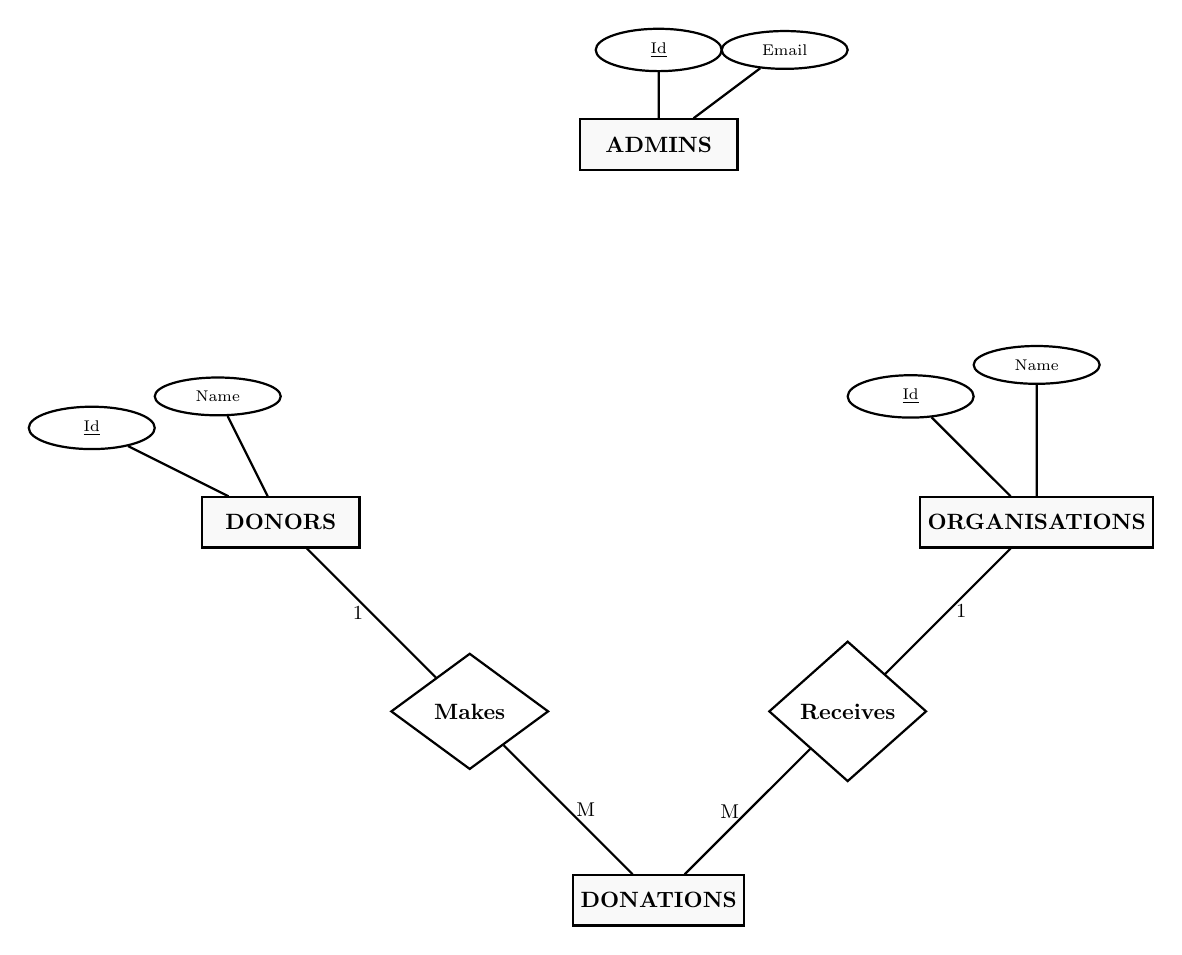
\begin{tikzpicture}[>=stealth, font=\small, thick, scale=0.8, transform shape]
\tikzset{
    entity/.style={draw, rectangle, minimum width=2.5cm, minimum height=0.8cm, fill=gray!5, font=\bfseries, align=center},
    attribute/.style={draw, ellipse, minimum width=2cm, minimum height=0.6cm, fill=white, font=\scriptsize, align=center},
    relationship/.style={draw, diamond, minimum width=2.5cm, minimum height=1cm, fill=white, font=\bfseries, align=center}
}
\node[entity] (Admin) at (0, 8) {ADMINS};
\node[entity] (Donor) at (-6, 2) {DONORS};
\node[entity] (Org) at (6, 2) {ORGANISATIONS};
\node[entity] (Donation) at (0, -4) {DONATIONS};
\node[relationship] (Makes) at (-3, -1) {Makes};
\node[relationship] (Receives) at (3, -1) {Receives};
\draw[-] (Donor) -- (Makes) node[midway, left] {1}; \draw[-] (Makes) -- (Donation) node[midway, right] {M};
\draw[-] (Org) -- (Receives) node[midway, right] {1}; \draw[-] (Receives) -- (Donation) node[midway, left] {M};
\node[attribute] (A1) at (0, 9.5) {\underline{Id}}; \node[attribute] (A2) at (2, 9.5) {Email}; \draw[-] (Admin) -- (A1); \draw[-] (Admin) -- (A2);
\node[attribute] (D1) at (-9, 3.5) {\underline{Id}}; \node[attribute] (D2) at (-7, 4) {Name}; \draw[-] (Donor) -- (D1); \draw[-] (Donor) -- (D2);
\node[attribute] (O1) at (4, 4) {\underline{Id}}; \node[attribute] (O2) at (6, 4.5) {Name}; \draw[-] (Org) -- (O1); \draw[-] (Org) -- (O2);
\end{tikzpicture}
}
\end{figure}

\newpage
% ---------------------------------------------------------
\section{Data Flow Diagram (Level 0 - Context)}
% -------------------------
\begin{figure}[htbp]
\centering
\resizebox{0.85\textwidth}{!}{
\begin{tikzpicture}[>=Latex, entity/.style={draw, rectangle, minimum width=3cm, minimum height=1.2cm, thick}, process/.style={draw, circle, minimum width=3.5cm, thick}, flow/.style={->, thick, font=\scriptsize}]
\node[process] (System) at (0,0) {0.0\\Social Help\\System};
\node[entity] (Donor) at (-7, 0) {Donor};
\node[entity] (Org) at (7, 0) {Organisation};
\node[entity] (Admin) at (0, 6) {Admin};
\draw[flow] ($(Donor.east)+(0,0.3)$) -- ($(System.west)+(0,0.3)$) node[midway, above] {Donations};
\draw[flow] ($(System.west)+(0,-0.3)$) -- ($(Donor.east)+(0,-0.3)$) node[midway, below] {Receipts};
\draw[flow] ($(Org.west)+(0,0.3)$) -- ($(System.east)+(0,0.3)$) node[midway, above] {Requirements};
\draw[flow] ($(System.east)+(0,-0.3)$) -- ($(Org.west)+(0,-0.3)$) node[midway, below] {Donor Info};
\draw[flow] ($(Admin.south)+(-0.3,0)$) -- ($(System.north)+(-0.3,0)$) node[midway, left] {Moderation};
\draw[flow] ($(System.north)+(0.3,0)$) -- ($(Admin.south)+(0.3,0)$) node[midway, right] {Reports};
\end{tikzpicture}
}
\end{figure}

\newpage
% ---------------------------------------------------------
\section{Data Flow Diagram (Level 1 - First Level)}
% -------------------------
\begin{figure}[htbp]
\centering
\resizebox{0.8\textwidth}{!}{
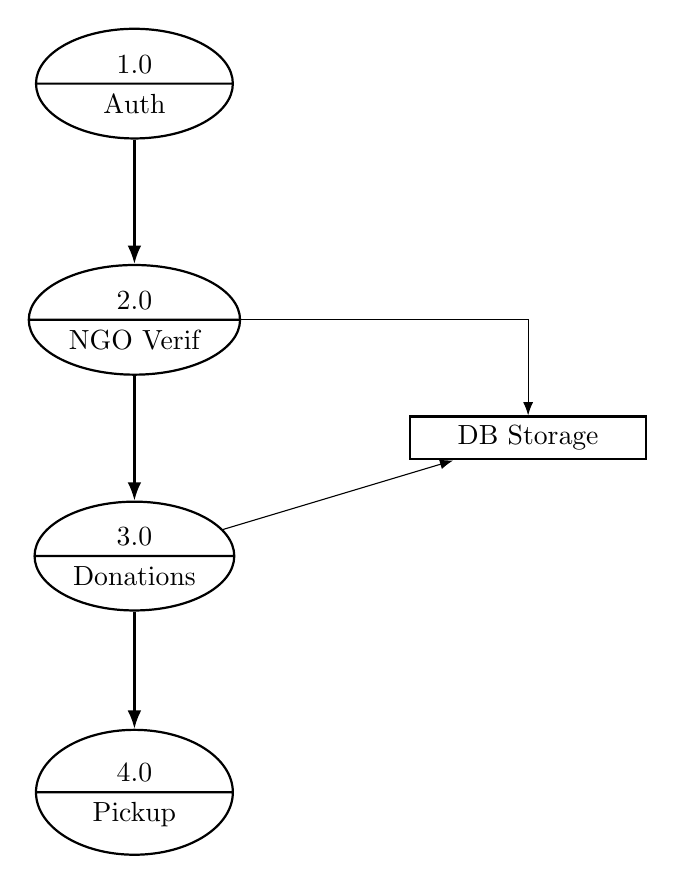
\begin{tikzpicture}[>=Latex, process/.style={ellipse split, draw, minimum width=2.5cm, thick}, datastore/.style={draw, minimum width=3cm, thick}]
\node[process] (P1) at (0, 0) {1.0 \nodepart{lower} Auth};
\node[process] (P2) at (0, -3) {2.0 \nodepart{lower} NGO Verif};
\node[process] (P3) at (0, -6) {3.0 \nodepart{lower} Donations};
\node[process] (P4) at (0, -9) {4.0 \nodepart{lower} Pickup};
\draw[->, thick] (P1) -- (P2); \draw[->, thick] (P2) -- (P3); \draw[->, thick] (P3) -- (P4);
\node[datastore] (D1) at (5, -4.5) {DB Storage};
\draw[->] (P2) -| (D1); \draw[->] (P3) -- (D1);
\end{tikzpicture}
}
\end{figure}

\newpage
% ---------------------------------------------------------
\section{Sequence Diagram (Donation Lifecycle)}
% -------------------------
\begin{figure}[htbp]
\centering
\resizebox{0.9\textwidth}{!}{
\begin{tikzpicture}[>=Latex, font=\small, thick]
\node[draw, rectangle, minimum width=2.5cm] (U) at (0,0) {UI};
\node[draw, rectangle, minimum width=2.5cm] (D) at (5,0) {Donor};
\node[draw, rectangle, minimum width=2.5cm] (S) at (10,0) {System};
\draw[dashed] (0,-0.5) -- (0,-6); \draw[dashed] (5,-0.5) -- (5,-6); \draw[dashed] (10,-0.5) -- (10,-6);
\draw[->] (0,-1.5) -- (5,-1.5) node[midway, above] {Donate()};
\draw[->] (5,-2.5) -- (10,-2.5) node[midway, above] {Save()};
\draw[<-, dashed] (5,-4) -- (10,-4) node[midway, above] {Success};
\draw[<-, dashed] (0,-5) -- (5,-5) node[midway, above] {Confirm};
\end{tikzpicture}
}
\end{figure}

\newpage
% ---------------------------------------------------------
\section{Activity Diagram (Workflow)}
% -------------------------
\begin{figure}[htbp]
\centering
\resizebox{0.6\textwidth}{!}{
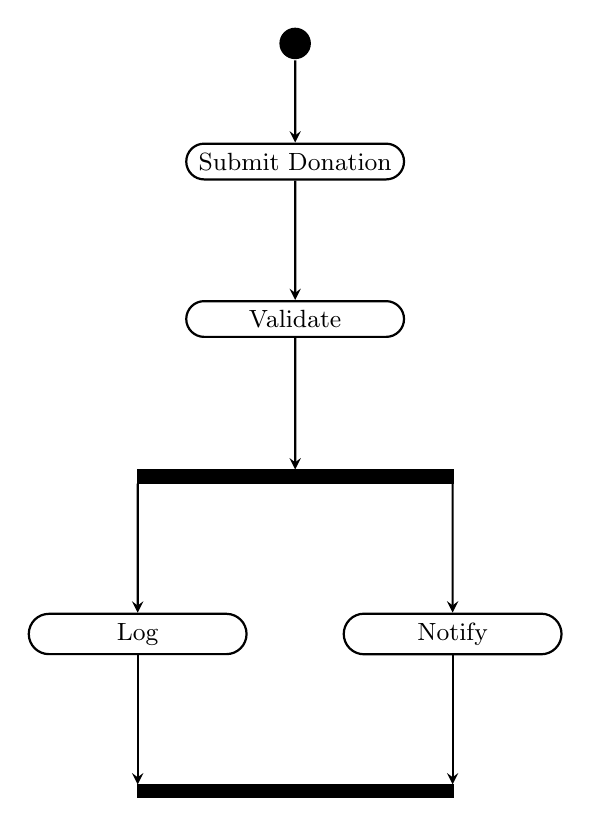
\begin{tikzpicture}[>=stealth, font=\small, thick]
\tikzset{act/.style={draw, rounded rectangle, minimum width=3cm, fill=white}, sync/.style={draw, fill=black, rectangle, minimum height=0.15cm, inner sep=0}, init/.style={fill=black, circle, minimum size=0.4cm}}
\node[init] (S) at (0,0) {};
\node[act] (A1) at (0,-1.5) {Submit Donation};
\node[act] (A2) at (0,-3.5) {Validate};
\node[sync, minimum width=4cm] (F) at (0,-5.5) {};
\node[act] (T1) at (-2, -7.5) {Log}; \node[act] (T2) at (2, -7.5) {Notify};
\node[sync, minimum width=4cm] (J) at (0,-9.5) {};
\draw[->] (S) -- (A1); \draw[->] (A1) -- (A2); \draw[->] (A2) -- (F);
\draw[->] (F.south -| T1) -- (T1); \draw[->] (F.south -| T2) -- (T2);
\draw[->] (T1.south) -- (J.north -| T1); \draw[->] (T2.south) -- (J.north -| T2);
\end{tikzpicture}
}
\end{figure}

\newpage
% ---------------------------------------------------------
\section{State Diagram (Post-Request Analysis)}
% -------------------------
\begin{figure}[htbp]
\centering
\resizebox{0.8\textwidth}{!}{
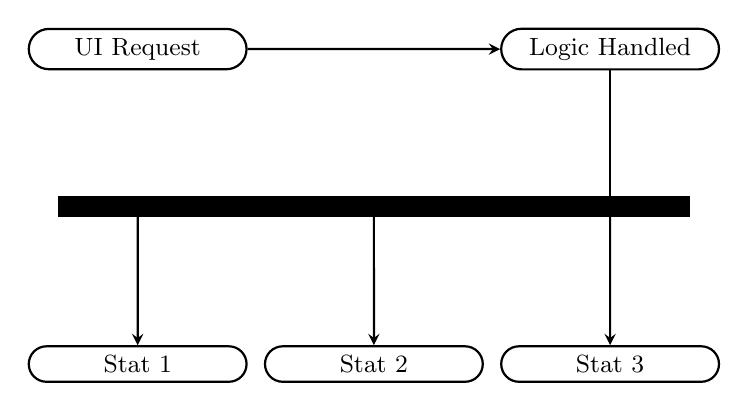
\begin{tikzpicture}[>=stealth, font=\small, thick]
\tikzset{act/.style={draw, rounded rectangle, minimum width=3cm}, sync/.style={draw, fill=black, rectangle, minimum height=0.15cm}}
\node[act] (A) at (0,0) {UI Request};
\node[act] (B) at (6,0) {Logic Handled};
\node[sync, minimum width=8cm] (F) at (3,-2) {};
\node[act] (C1) at (0,-4) {Stat 1}; \node[act] (C2) at (3,-4) {Stat 2}; \node[act] (C3) at (6,-4) {Stat 3};
\draw[->] (A) -- (B); \draw[->] (B) |- (F);
\draw[->] (F.south -| C1) -- (C1); \draw[->] (F.south -| C2) -- (C2); \draw[->] (F.south -| C3) -- (C3);
\end{tikzpicture}
}
\end{figure}

\newpage
% ---------------------------------------------------------
\section{Object Diagram (Runtime Instance)}
% -------------------------
\begin{figure}[htbp]
\centering
\resizebox{0.9\textwidth}{!}{
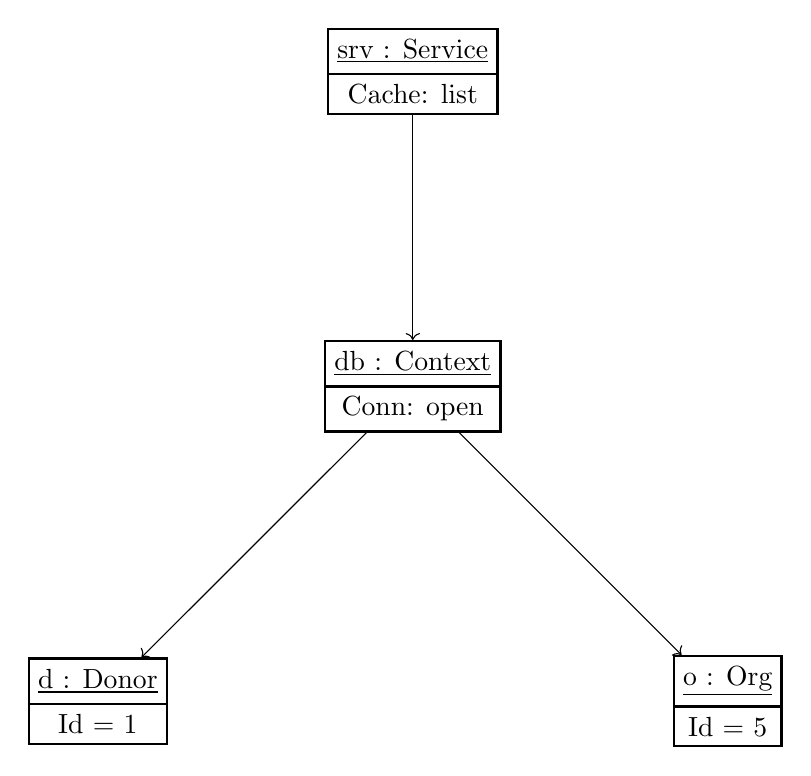
\begin{tikzpicture}[obj/.style={draw, rectangle split, rectangle split parts=2, fill=white, thick}]
\node[obj] (S) at (0,0) {\underline{srv : Service} \nodepart{second} Cache: list};
\node[obj] (D) at (0,-4) {\underline{db : Context} \nodepart{second} Conn: open};
\node[obj] (E1) at (-4,-8) {\underline{d : Donor} \nodepart{second} Id = 1};
\node[obj] (E2) at (4,-8) {\underline{o : Org} \nodepart{second} Id = 5};
\draw[->] (S) -- (D); \draw[->] (D) -- (E1); \draw[->] (D) -- (E2);
\end{tikzpicture}
}
\end{figure}

\newpage
% ---------------------------------------------------------
\section{Component Diagram}
% -------------------------
\begin{figure}[htbp]
\centering
\resizebox{0.8\textwidth}{!}{
\begin{tikzpicture}
\tikzset{comp/.style={draw, rectangle, minimum width=3cm, minimum height=1.5cm, fill=white}}
\node[comp] (C1) at (0,0) {Web UI};
\node[comp] (C2) at (5,0) {Business API};
\node[comp] (C3) at (5,-3) {Data Access};
\draw[->, dashed] (C1) -- (C2); \draw[->, dashed] (C2) -- (C3);
\end{tikzpicture}
}
\end{figure}

\newpage
% ---------------------------------------------------------
\section{Deployment Diagram}
% -------------------------
\begin{figure}[htbp]
\centering
\resizebox{0.8\textwidth}{!}{
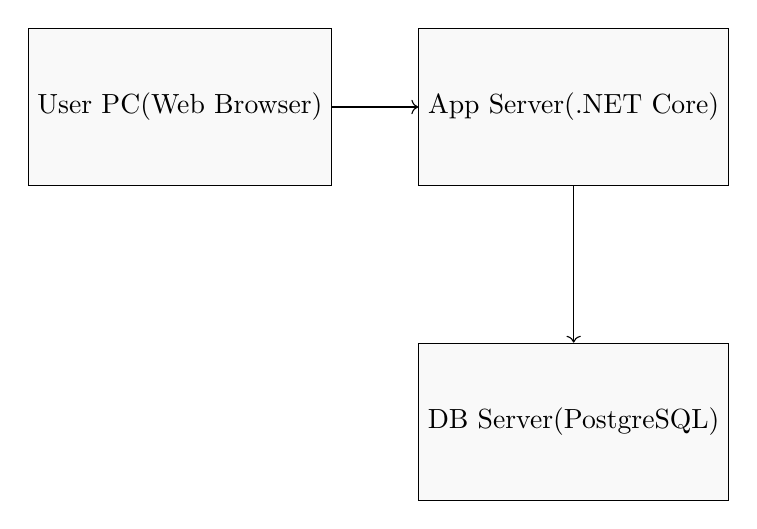
\begin{tikzpicture}
\tikzset{node/.style={draw, rectangle, minimum width=3cm, minimum height=2cm, fill=gray!5}}
\node[node] (N1) at (0,0) {User PC\\(Web Browser)};
\node[node] (N2) at (5,0) {App Server\\(.NET Core)};
\node[node] (N3) at (5,-4) {DB Server\\(PostgreSQL)};
\draw[->] (N1) -- (N2); \draw[->] (N2) -- (N3);
\end{tikzpicture}
}
\end{figure}

\newpage
% ---------------------------------------------------------
\section{Functional Decomposition Diagram (FDD)}
% -------------------------
\begin{figure}[htbp]
\centering
\resizebox{0.8\textwidth}{!}{
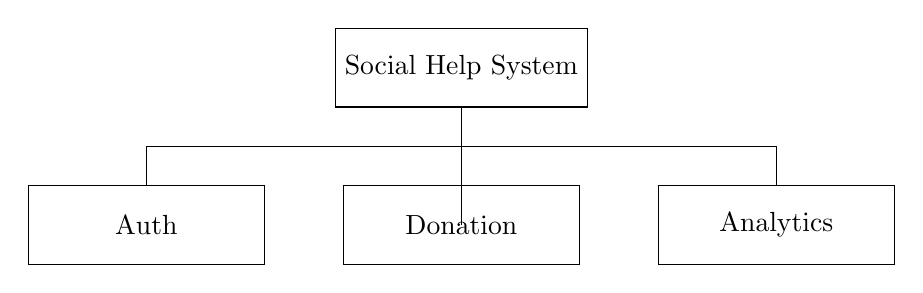
\begin{tikzpicture}[block/.style={draw, rectangle, minimum width=3cm, minimum height=1cm, align=center}]
\node[block] (Main) at (0,0) {Social Help System};
\node[block] (M1) at (-4,-2) {Auth};
\node[block] (M2) at (0,-2) {Donation};
\node[block] (M3) at (4,-2) {Analytics};
\draw[-] (Main) -- (0,-1) -- (-4,-1) -- (M1);
\draw[-] (Main) -- (0,-2); \draw[-] (0,-1) -- (4,-1) -- (M3);
\end{tikzpicture}
}
\end{figure}

\end{document}
